\documentclass[14pt]{beamer}


\usepackage{color}
\usepackage{tikz}


\mode<presentation>
{
\usetheme{AlpesLasers}
\setbeamercovered{transparent}
  %\setbeamertemplate{footline}[frame number] 
  %\setbeamertemplate{navigation symbols}{ 
  %\hskip 0.3cm
  %\insertframenumber / \inserttotalframenumber  % <<< frame #
  %\insertpagenumber / \insertpresentationendpage % <<< page #
%} 
}

% font definitions, try \usepackage{ae} instead of the following
% three lines if you don't like this look
\usepackage{listings}
\lstloadlanguages{python}

\usepackage{mathptmx}
\usepackage[scaled=.90]{helvet}
\usepackage{courier}
\usepackage[T1]{fontenc}
\usepackage[english]{babel}
\usepackage[latin1]{inputenc}
\title{Simulations for Alpes Lasers SA}
\subtitle{\includegraphics[width=2cm]{europe}}
\author{St\'ephane Poss}
\date{July 8th, 2015}
% This is only inserted into the PDF information catalog. Can be left
% out.
\subject{PYTHON}

\begin{document}
\begin{frame}[plain]
\titlepage
\end{frame}

\begin{frame}
\frametitle{Outline}
\begin{itemize}
\item Background
\item Current project
\item Secondment
\end{itemize}
\end{frame}

\begin{frame}
\frametitle{2003-2009}
\centering
\includegraphics[width=\textwidth]{marseille}
\end{frame}

\begin{frame}
\centering
\includegraphics[width=\textwidth]{CPPM_img1}
\end{frame}

\begin{frame}
\centering
\includegraphics[width=\textwidth]{Lhcbview}
\end{frame}

\begin{frame}
\centering
\includegraphics[width=\textwidth]{CPasymetry}
\end{frame}

\begin{frame}
\centering
\includegraphics[width=0.5\textwidth]{these}

\end{frame}

\begin{frame}
\frametitle{2010-2013}
\centering
\includegraphics[width=0.5\textwidth]{CERN}
\includegraphics[width=0.5\textwidth]{CLIC}

\end{frame}

\begin{frame}
\centering
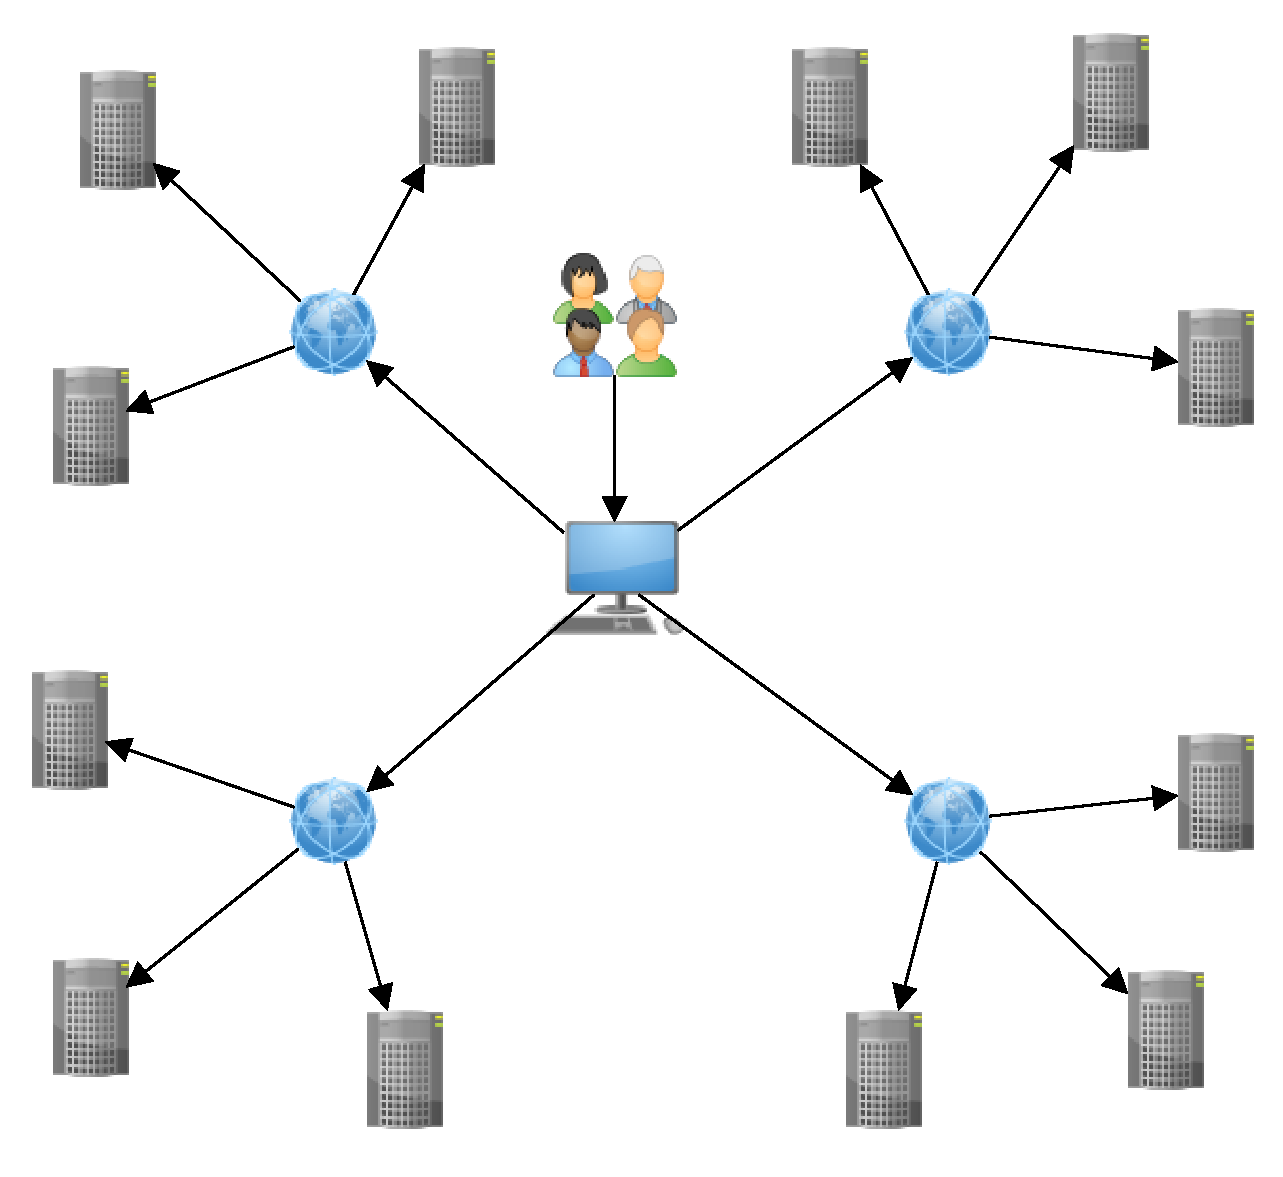
\includegraphics[width=0.7\textwidth]{network}

\end{frame}

\begin{frame}
\centering
\includegraphics[width=0.5\textwidth]{CLICDR}

\end{frame}

\begin{frame}
\frametitle{Current project: Alpes Lasers}
Ojectives:
\begin{itemize}
\item Design and implement a distributed computing solution for the simulation needs of the company
\item Provide convenient tools to run the different simulation softwares
\end{itemize}
\end{frame}

\begin{frame}
\centering
\includegraphics[width=\textwidth]{Architecture1}

\end{frame}

\begin{frame}
\frametitle{Presentations}
\begin{itemize}
\item DIRAC user community meeting 2014, 2015
\item Internal Journal club
\end{itemize}
\end{frame}

\begin{frame}
\frametitle{Secondment}
March 31st - April 12th: Univ Paris-Diderot, Cristiano Ciutti:
\begin{itemize}
\item Presentation of computing tools: emphasis on PYTHON
\item Discussions on computing methods
\item Implementation of utility for remote matlab execution
\end{itemize}
\end{frame}


\end{document}